\documentclass[lettersize,journal]{IEEEtran}

\usepackage{amsmath,amsfonts,amssymb}
\usepackage{array}
\usepackage{stfloats}
\usepackage{url}
\usepackage{graphicx}
\usepackage{cite}
% \rev{} marks a number new or changed in Draft_14; each one is traced in
% Plans/Draft_14_numbers.md. It typesets as its argument.
\newcommand{\rev}[1]{#1}
% \prelim{} marks a number from a reduced-size run (Fig. 7 sweep at 1000
% trials per cell, radius and mechanism runs at 2000) awaiting the overnight
% 10^4 runs listed in overnight_runs.txt. It prints blue.
\usepackage{xcolor}
\newcommand{\prelim}[1]{\textcolor{blue}{#1}}
\hyphenation{op-tical net-works semi-conduc-tor IEEE-Xplore}
\def\BibTeX{{\rm B\kern-.05em{\sc i\kern-.025em b}\kern-.08em
    T\kern-.1667em\lower.7ex\hbox{E}\kern-.125emX}}

\urlstyle{same}

% Float spacing: IEEEtran defaults leave generous gaps around floats.
% Tightened to recover vertical space without altering figure content.
\setlength{\textfloatsep}{4pt plus 1pt minus 1pt}
\setlength{\floatsep}{6pt plus 2pt minus 2pt}
\setlength{\intextsep}{6pt plus 2pt minus 2pt}
\setlength{\dbltextfloatsep}{4pt plus 1pt minus 1pt}
\setlength{\dblfloatsep}{6pt plus 2pt minus 2pt}
\setlength{\abovecaptionskip}{3pt}
% Float packing: IEEEtran's defaults reserve a large fraction of each
% column for text, which strands whitespace on figure-heavy pages.
% Raising the float fractions lets LaTeX fill those pages properly.
\renewcommand{\topfraction}{0.95}
\renewcommand{\bottomfraction}{0.95}
\renewcommand{\textfraction}{0.05}
\renewcommand{\floatpagefraction}{0.85}
\renewcommand{\dbltopfraction}{0.95}
\renewcommand{\dblfloatpagefraction}{0.85}
\setlength{\belowcaptionskip}{0pt}

\begin{document}

\title{Second-Order Cooperative Field Estimation and Tracking of Coherent Flow Structures Using Multirobot Systems}

\author{Christopher Waight and Christopher A. Kitts,~\IEEEmembership{Senior Member,~IEEE}
\thanks{C. Waight is a PhD Candidate in the Robotic Systems Laboratory, Department of Mechanical Engineering, Santa Clara University, Santa Clara, CA 95053 USA (e-mail: cwaight@scu.edu)}
\thanks{C. A. Kitts is Professor and Director of the Robotic Systems Laboratory, Department of Mechanical Engineering, Santa Clara University, Santa Clara, CA 95053 USA (e-mail: ckitts@scu.edu)}
}
\markboth{IEEE Systems Journal}%
{Waight and Kitts: Second-Order Cooperative Field Estimation and Tracking of Coherent Flow Structures}

\maketitle

\begin{abstract}
A cluster of robots that measures a flow as it moves can steer itself
toward the curves that organize that flow. This paper develops adaptive
navigation for two short-term transport structures, the curves across
which water masses separate and the curves along which floating material
collects. Existing robotic trackers of these
structures pre-straddle them before tracking begins and either commit to
the structure's identity or accumulate an estimate over a finite
integration horizon to determine the type. We show that synchronized
measurements from six robots recover a second-order polynomial model of
the local flow. From this model we compute two scalar fields, the Jacobian
determinant field $D$ and the smaller rate-of-strain eigenvalue field
$s_1$, whose trenches lie closest to these structures where strain
dominates rotation. Two adaptive navigation primitives, the $D$ tracker and the
$s_1$ tracker, each locate the nearest trench of their field and navigate
to and along it from instantaneous measurements, with no integration
horizon or pre-straddling requirement. Monte Carlo analysis
shows that the $D$ tracker withstands more measurement noise from every
tested start. However, the $s_1$ tracker is built from objective
quantities and holds its path when the observer rotates, while the $D$
tracker does not. On Santa Barbara Channel radar currents, both primitives
acquire the dominant transport corridor, but under small changes to the
start only the $D$ tracker keeps its downstream direction.

\end{abstract}

\begin{IEEEkeywords}
Mobile Robots, Multirobot Systems, Adaptive Navigation, Coherent
Structures, Rate of Strain, Objectivity, Cooperative Estimation,
Cluster Space Control
\end{IEEEkeywords}

\section{Introduction}


\IEEEPARstart{M}{ultirobot} systems (MRS) offer redundancy, increased
throughput, and cooperative capabilities a single robot cannot produce, and have
succeeded across land, sea, air, and space \cite{1,2}. In adaptive
navigation (AN), a vehicle or group of vehicles modifies its trajectory in
real time from measurements taken while moving \cite{3}. A single vehicle
must move to sense a gradient, which costs time and misleads in a changing
field, while an MRS samples many points at once.


AN in scalar fields is well developed. \"{O}gren, Fiorelli, and Leonard
established cooperative gradient climbing with a formation of mobile
sensors using plane fitting \cite{4}. Bri\~{n}\'{o}n-Arranz, Renzaglia, and Schenato
extended the fit to recover the Hessian from five robots on a ring plus
one at the center \cite{5}. Kitts, McDonald, and
Neumann developed primitives for extrema finding, contour following,
ridge/trench following, and saddle point station keeping \cite{3}, and
verified ridge, trench, saddle, and front tracking on an indoor testbed
\cite{6,7}.

Some flows are better described as vector fields, which carry features a
scalar map cannot. Critical points, such as sinks, sources, and vortices,
can model convergence zones \cite{8} and subsurface leaks \cite{9}. In
\cite{10} a three-robot cluster located and typed a nearby critical point
from a linear fit of simultaneous velocity measurements and navigated to
and around it.

A vector field also carries well-defined curves. In a dynamic ocean flow some of these are coherent structures, boundaries that influence where floating material such as debris and larvae accumulates or separates \cite{11,12}.
Coherent structures are typically identified in one of two ways. The
first finds Lagrangian coherent structures (LCS) \cite{13}, typically as
ridges of the finite-time Lyapunov exponent (FTLE) field \cite{14}. The
second uses instantaneous Eulerian criteria, such as the Okubo-Weiss
parameter, which partition the flow by the local velocity gradient alone
\cite{8,15}. This instantaneous approach has been generalized to three
dimensions \cite{16}, refined to second order \cite{17}, and applied at
scale in mesoscale eddy censuses \cite{18}. Their tradeoffs remain under
study \cite{19,20,21,22}.


Mapping these curves tells a search where floating material has gathered
\cite{12}, and ocean sampling campaigns already steer vehicles toward
dynamic features such as fronts \cite{23,24,25}. Without adaptive
navigation, a large fleet must survey the basin and reconstruct the
structures offline; adaptive navigation maps them locally with one small
cluster.


Michini et al. travel along a presumed stable or
unstable manifold with three robots using only local velocity
measurements \cite{26}, an approach based on the PIM triple procedure
that its authors extend to larger teams \cite{27} and to robots in a flow
tank \cite{28}. The saddle point is addressed by neither the
controller nor its analysis.
Kularatne and Hsieh confirm an attracting boundary by computing the local
FTLE field on board, at the cost of a nonzero integration horizon
\cite{29}.
Their analysis assumes that the robots start straddling the structure
\cite{26,27} or that the center robot starts on it \cite{29}.


This paper shows that a second-order polynomial fit of the local flow can
acquire and track such a structure from instantaneous measurements. The
contributions are as follows.
First, a cooperative estimator recovers the local quadratic model of
a two-component field from one synchronized set of measurements across six
robots, the fewest that can, extending the scalar gradient and Hessian
estimation of \cite{5} to both components of a vector field. Second, two surrogate fields computed from that fit,
the determinant field $D$ and the smaller strain eigenvalue field $s_1$,
turn the search for a separatrix into the search for a trench, the kind of
feature the scalar primitives of \cite{3} follow. Third, two AN
primitives, the $D$ tracker and the $s_1$ tracker, navigate to the trench
from a start that does not straddle it and ride along it. Finally, a
comparison shows that the $D$ tracker tolerates more measurement noise,
while the $s_1$ tracker is built from objective quantities, so that
observers rotating relative to each other agree on its path except where
its tangent swaps eigenvector. A rotation-to-strain ratio from the same
fit indicates when either trench likely marks a separatrix.

Both primitives run on a simulated double gyre, three variants, and
measured Santa Barbara Channel radar currents.

\section{Second-Order Field Estimation}

\subsection{Quadratic Field Estimation}

A planar vector field assigns a velocity $\mathbf{v}(\mathbf{p}) =
(u(\mathbf{p}), v(\mathbf{p}))$ to each position in space $\mathbf{p} = (x, y)$.
The critical point estimator of \cite{10} fits a plane to each
component of the vector field and solves for the point where $\mathbf{v} = \mathbf{0}$. 

In this work, we extend the linear approximation to the second-order Taylor expansion about the
centroid $\mathbf{p}_c$, with $x$ and $y$ measured from $\mathbf{p}_c$.

\begin{align}
    u(\mathbf{p}) &= a_1 + a_2 x + a_3 y
        \nonumber \\
        &\quad + a_4 xy + \tfrac{1}{2} a_5 x^2 + \tfrac{1}{2} a_6 y^2
        + \mathcal{O}(\|\mathbf{p}\|^3),
        \label{eq:quad_model_u} \\
    v(\mathbf{p}) &= b_1 + b_2 x + b_3 y
        \nonumber \\
        &\quad + b_4 xy + \tfrac{1}{2} b_5 x^2 + \tfrac{1}{2} b_6 y^2
        + \mathcal{O}(\|\mathbf{p}\|^3),
        \label{eq:quad_model_v}
\end{align}
where $\mathcal{O}(\|\mathbf{p}\|^3)$ is the truncation error.
The twelve coefficients are constants, and the one-half factors make each
one a derivative of the flow at $\mathbf{p}_c$. The flow itself is $a_1$,
$a_2$ and $a_3$ are $\partial u/\partial x$ and $\partial u/\partial y$,
and $a_4$, $a_5$, and $a_6$ are $\partial^2 u/\partial x\partial y$,
$\partial^2 u/\partial x^2$, and $\partial^2 u/\partial y^2$, with
$b_1, \ldots, b_6$ the same for $v$.

To estimate these coefficients with robot positions $\mathbf{p}_i = (x_i,
y_i)$, we define the quadratic basis vector
\begin{equation}
    \boldsymbol{\phi}(\mathbf{p}) =
    \bigl[\,1, \; x, \; y, \; xy, \;
    \tfrac{1}{2}x^2, \; \tfrac{1}{2}y^2\,\bigr]^\top.
\end{equation}



Stacking the $n$ basis vectors row-wise gives us the $n \times 6$ formation matrix $\boldsymbol{\Phi}$, and the coefficient estimates $\hat{\boldsymbol{\theta}}_u$ and $\hat{\boldsymbol{\theta}}_v$ solve
\begin{equation}
\boldsymbol{\Phi}\,\hat{\boldsymbol{\theta}}_u = \mathbf{m}_u, \qquad
\boldsymbol{\Phi}\,\hat{\boldsymbol{\theta}}_v = \mathbf{m}_v,
\label{eq:solve}
\end{equation}
where $\mathbf{m}_u = [u_1, \ldots, u_n]^\top$ and
$\mathbf{m}_v = [v_1, \ldots, v_n]^\top$ collect the components $u_i$
and $v_i$ that robot $i$ measures.

\subsection{Minimality}
\label{sec:minimality}

Six robots is the minimum for recovery of the unconstrained local
quadratic model from one set of instantaneous measurements, the
second-order counterpart of the three-robot minimum for a linear fit
\cite[Prop.~1]{10}. Each robot contributes one equation per component of
(\ref{eq:solve}), and each system has six unknowns. With five robots or
fewer, a method must either return a family of solutions or impose a
prior such as $\nabla\cdot\mathbf{v} = 0$, which would bias every
coefficient of a horizontal surface current, since such currents are not
divergence-free. Six robots suffice provided $\boldsymbol{\Phi}$ is
nonsingular, and more than six need $\boldsymbol{\Phi}$ to have full
column rank for least squares. Either condition fails exactly when the
robots lie on a common conic, so a ring formation is degenerate at any
size. A fit from more than six robots also leaves a residual, which
carries both the measurement noise and the truncation error.

We use the pentagon-plus-center formation of \cite{5} throughout. It is
the smallest uniform ring plus center on which \cite{5} recovers a scalar
Hessian exactly for quadratic signals at any orientation, and the same
symmetry makes the noise gains of the fit here independent of heading.


\subsection{Estimator Sensitivity}
\label{sec:sensitivity}

Three things limit the fit: the formation, the noise on each reading,
and the error in each robot's position.

\subsubsection{Formation}
The 2-norm condition number $\kappa(\boldsymbol{\Phi})$ indicates how much
the fit amplifies noise. On the radius-normalized $\boldsymbol{\Phi}$, with
each column of order $q$ divided by $\rho^{\,q}$ for formation radius
$\rho$, the pentagon-plus-center formation gives
$\kappa(\boldsymbol{\Phi}) = 8.26$ at every radius. The formation's size
changes instead how much noise reaches each coefficient. A coefficient of order $q$ is recovered
from differences in readings across the footprint divided by
$\rho^{\,q}$, so its noise scales as $\rho^{-q}$. A larger formation
therefore suppresses noise most in the second-order terms, but it also
increases the truncation error, since the ring robots sit at
$\|\mathbf{p}\| = \rho$. Moving the center robot out to $0.99\rho$
places all six robots within $0.6\%$ of a common circle and raises
$\kappa(\boldsymbol{\Phi})$ to $564$, so the fit degrades smoothly near
a conic.

\subsubsection{Measurement Noise}
Every robot reads the current with its own sensor, and each fit uses only
the readings of its own cycle. The noise in one fit is therefore
independent across robots and across cycles. It is modeled as additive on
each reading, $u_i^m = u(\mathbf{p}_i) + \eta_i^u$ and
$v_i^m = v(\mathbf{p}_i) + \eta_i^v$ with
$\eta \sim \mathcal{N}(0, \sigma_{uv}^2)$. The fit is linear in the
readings, so the noise reaches the coefficients as
$\boldsymbol{\Phi}^{-1}\boldsymbol{\eta}$, where $\boldsymbol{\eta}$
stacks the noise of the six robots. It adds no bias, and its covariance is
$\mathrm{Cov}(\hat{\boldsymbol{\theta}}) =
\sigma_{uv}^2(\boldsymbol{\Phi}^\top\boldsymbol{\Phi})^{-1}$ for each of
$\hat{\boldsymbol{\theta}}_u$ and $\hat{\boldsymbol{\theta}}_v$, which
are independent. For the pentagon-plus-center formation its diagonal does
not depend on heading. A reading noise $\sigma_{uv}$ gives the flow estimate a standard deviation
$\sigma_{uv}$, each first derivative $\rev{0.632}\,\sigma_{uv}/\rho$, the
mixed second derivative $\rev{1.265}\,\sigma_{uv}/\rho^2$, and each pure
second derivative $\rev{2.53}\,\sigma_{uv}/\rho^2$.

\subsubsection{Position Noise}
A robot with position error
$\boldsymbol{\xi}_i \sim \mathcal{N}(\mathbf{0}, \sigma_p^2\mathbf{I})$
samples the field at $\mathbf{p}_i + \boldsymbol{\xi}_i$, but the fit is
built from its nominal position $\mathbf{p}_i$. The formation matrix is
therefore wrong by $\Delta\boldsymbol{\Phi}$, whose row $i$ is
$\boldsymbol{\phi}(\mathbf{p}_i + \boldsymbol{\xi}_i)^{\top} -
\boldsymbol{\phi}(\mathbf{p}_i)^{\top}$. Under the quadratic model the
measurements are
$\mathbf{m}_u = (\boldsymbol{\Phi} + \Delta\boldsymbol{\Phi})
\boldsymbol{\theta}_u$, and the fit returns
\begin{equation}
    \hat{\boldsymbol{\theta}}_u = \boldsymbol{\theta}_u
        + \boldsymbol{\Phi}^{-1}\Delta\boldsymbol{\Phi}\,
          \boldsymbol{\theta}_u ,
    \label{eq:pos_noise}
\end{equation}
and likewise for $\hat{\boldsymbol{\theta}}_v$. To first order, entry
$i$ of $\Delta\boldsymbol{\Phi}\,\boldsymbol{\theta}_u$ is
$\nabla u \cdot \boldsymbol{\xi}_i$, the change in $u$ across the
displacement. This error vanishes in uniform flow and grows with the
local gradient, so unlike measurement noise it depends on the field.



\subsection{Eulerian Surrogates}
\label{sec:surrogates}

Lagrangian methods locate coherent structures by integrating particle
trajectories over a finite time window \cite{13,14}. This paper instead
reads them from the instantaneous geometry of the velocity field, as
Eulerian coherent structures \cite{20}. Two fields computed from the
six-robot fit can mark the separatrix. The first is the determinant of the velocity
gradient, and the second is the smaller eigenvalue of its symmetric
part.

\subsubsection{Determinant Field}
The fitted coefficients define the velocity gradient
$\mathbf{J} = \nabla\mathbf{v}$ at every point of the footprint. Differentiating the quadratic model gives a Jacobian whose
entries are affine in position,
\begin{equation}
    \hat{\mathbf{J}}(\mathbf{p}) =
    \begin{bmatrix}
        \hat{a}_2 + \hat{a}_5 x + \hat{a}_4 y &
        \hat{a}_3 + \hat{a}_4 x + \hat{a}_6 y \\
        \hat{b}_2 + \hat{b}_5 x + \hat{b}_4 y &
        \hat{b}_3 + \hat{b}_4 x + \hat{b}_6 y
    \end{bmatrix}.
    \label{eq:Jhat}
\end{equation}
The determinant $\hat{D}(\mathbf{p}) = \det\hat{\mathbf{J}}(\mathbf{p})$
is therefore exactly quadratic over the footprint. Its value, gradient,
and Hessian at the centroid are polynomials in the coefficients. The
value is $\hat{D}_0 = \hat{a}_2\hat{b}_3 - \hat{a}_3\hat{b}_2$, and the
gradient is
\begin{equation}
    \hat{\mathbf{g}}_0 =
    \begin{bmatrix}
        \hat{a}_5\hat{b}_3 + \hat{a}_2\hat{b}_4 - \hat{a}_4\hat{b}_2 - \hat{a}_3\hat{b}_5 \\
        \hat{a}_4\hat{b}_3 + \hat{a}_2\hat{b}_6 - \hat{a}_6\hat{b}_2 - \hat{a}_3\hat{b}_4
    \end{bmatrix}.
    \label{eq:grad_det}
\end{equation}
The Hessian is
\begin{equation}
    \hat{\mathbf{H}}_{D,0} =
    \begin{bmatrix}
        2(\hat{a}_5\hat{b}_4 - \hat{a}_4\hat{b}_5) &
        \hat{a}_5\hat{b}_6 - \hat{a}_6\hat{b}_5 \\
        \hat{a}_5\hat{b}_6 - \hat{a}_6\hat{b}_5 &
        2(\hat{a}_4\hat{b}_6 - \hat{a}_6\hat{b}_4)
    \end{bmatrix},
    \label{eq:hess_det}
\end{equation}
which is constant over the footprint.

For incompressible flow the determinant is a negative multiple of the
Okubo-Weiss parameter \cite{8,15}, so the two carry the same partition of
the flow. Where $D < 0$ the flow is strain-dominated, and where $D > 0$
it is rotation-dominated.


\subsubsection{Strain Eigenvalue Field}
The second surrogate comes from the rate-of-strain tensor
$\hat{\mathbf{S}} = \tfrac{1}{2}(\hat{\mathbf{J}} + \hat{\mathbf{J}}^{\top})$,
the symmetric part of the same fitted Jacobian.
At the centroid its mean, deviatoric normal, and shear strain are
$\hat{\mu} = (\hat{a}_2 + \hat{b}_3)/2$,
$\hat{s}_n = (\hat{a}_2 - \hat{b}_3)/2$, and
$\hat{s}_s = (\hat{a}_3 + \hat{b}_2)/2$, and each is affine in position.
The eigenvalues of $\hat{\mathbf{S}}$ are
$\hat{s}_{1,2} = \hat{\mu} \mp \hat{r}$ with
$\hat{r} = \sqrt{\hat{s}_n^2 + \hat{s}_s^2}$. Their eigenvectors
$\mathbf{e}_1$ and $\mathbf{e}_2$ are the compression and stretching
directions, and the gradient of the smaller eigenvalue is
\begin{equation}
    \nabla\hat{s}_1 = \nabla\hat{\mu}
        - \frac{\hat{s}_n\nabla\hat{s}_n + \hat{s}_s\nabla\hat{s}_s}{\hat{r}},
    \label{eq:grad_s1}
\end{equation}
where the second-order coefficients give the constant gradients
\begin{equation}
    \begin{aligned}
        \nabla\hat{\mu} &= \tfrac{1}{2}(\hat{a}_5 + \hat{b}_4,\; \hat{a}_4 + \hat{b}_6), \\
        \nabla\hat{s}_n &= \tfrac{1}{2}(\hat{a}_5 - \hat{b}_4,\; \hat{a}_4 - \hat{b}_6), \\
        \nabla\hat{s}_s &= \tfrac{1}{2}(\hat{a}_4 + \hat{b}_5,\; \hat{a}_6 + \hat{b}_4).
    \end{aligned}
    \label{eq:grad_strain}
\end{equation}
The quotient stays bounded as $\hat{r} \to 0$ but its direction is
undefined at $\hat{r} = 0$, so the computation floors $\hat{r}$ at
$10^{-12}$. Unlike $\hat{D}$, $\hat{s}_1$ has no usable Hessian. It is an
affine function minus the norm of an affine map, so it is concave over the
footprint for every field and formation.

Serra and Haller define objective Eulerian coherent structures (OECS)
from these eigenvalues and eigenvectors \cite{20}. An attracting OECS is a
trench of $s_1$ tangent to $\mathbf{e}_2$, and floating material has been
seen at sea to collect on such curves \cite{12}. A repelling OECS is a
ridge of $s_2$ tangent to $\mathbf{e}_1$, where neighboring material
separates. In incompressible flow $s_2 = -s_1$, so repelling structures are
trenches of $s_1$ too, and one tracker rides both.

\subsubsection{Relation Between the Fields}
Both fields come from the same fitted Jacobian. With the vorticity
$\omega = \partial v/\partial x - \partial u/\partial y$, the Jacobian
splits into its mean, strain, and rotation parts, and the two fields become
\begin{equation}
    D = \mu^2 - r^2 + \tfrac{1}{4}\omega^2, \qquad s_1 = \mu - r.
    \label{eq:D_parts}
\end{equation}
In divergent flow, $D < 0$ therefore means that strain outweighs rotation
and divergence together. A trench of $D$ is a curve where strain most
outweighs rotation, and a trench of $s_1$ is a curve of strongest
instantaneous compression or stretching. Neither mentions streamlines, so
the trenches mark a separatrix only where the rotation on it is small
against the strain. The ratio $|\omega|/2r$ measures how small. A small
ratio is necessary rather than sufficient.

Where the vorticity vanishes, $\mathbf{J} = \mathbf{S}$ and
$D = s_1 s_2$, which is $-s_1^2$ in incompressible flow. The vorticity
also separates the two fields across observers. A frame rotating clockwise
at rate
$\Omega$, with rotation $\mathbf{Q}$, adds a uniform spin that raises
$\omega$ to $\omega + 2\Omega$. The strain tensor only co-rotates, so
$s_1$ is objective \cite{20}, while the determinant keeps the spin,
\begin{equation}
    D' = D + \Omega\,\omega + \Omega^2 .
    \label{eq:D_not_objective}
\end{equation}
Relatively rotating observers therefore disagree about where the
trenches of $D$ lie, and about $|\omega|/2r$, since the frame adds $2\Omega$
to $\omega$ but leaves $r$ unchanged.

\subsection{The Double-Gyre Example}
\label{sec:dg_example}

The double gyre is
a benchmark flow on which both fields mark the material transport structure
exactly, and every
quantity of interest has a closed form. The flow is two counter-rotating gyres in a
closed basin, separated by a separatrix that runs between two saddle points on
the basin walls. We use the steady member of the Shadden
family~\cite{14}, shifted from the canonical domain
$[0,2]\times[0,1]$ to $[-1,1]\times[-0.5,0.5]$ by $x_f = x + 1$,
$y_f = y + 0.5$ to center it on the origin. All double-gyre quantities are
non-dimensional. The field is
\begin{equation}
u = -\pi A \sin(\pi x_f)\cos(\pi y_f), \quad
v = \pi A \cos(\pi x_f)\sin(\pi y_f),
\label{eq:dg_u}
\end{equation}
with $A = 0.1$. The separatrix is $x = 0$, the saddles are
$\mathbf{p}_1^* = (0, -0.5)$ and $\mathbf{p}_2^* = (0, 0.5)$, and the gyre
centers $(\pm 0.5, 0)$.

The analytical Jacobian entries are
$u_x = -\pi^2 A \cos\pi x_f \cos\pi y_f = -v_y$ and
$u_y = \pi^2 A \sin\pi x_f \sin\pi y_f = -v_x$, with subscripts denoting
partial derivatives of the true field. The flow is therefore
incompressible, and its determinant and Hessian are
\begin{equation}
\begin{aligned}
D(\mathbf{p}) &= -\tfrac{1}{2}\pi^4 A^2 \left(\cos 2\pi x_f + \cos 2\pi y_f\right),\\
\mathbf{H}_D &= 2\pi^6 A^2
\begin{bmatrix} \cos 2\pi x_f & 0 \\ 0 & \cos 2\pi y_f \end{bmatrix}.
\end{aligned}
\label{eq:det_analytic_main}
\end{equation}
The landscape of $D$ forms a mountain pass over the separatrix
(Fig.~\ref{fig:dg_fields}(b)). Its peaks are the two gyre centers, where
rotation dominates and $D > 0$. Its lowest points are the flow saddles
$\mathbf{p}_1^*$ and $\mathbf{p}_2^*$, joined by a trench along the
separatrix that rises to a crest at the origin, where $D = 0$ and the
separatrix splits into an upper and a lower segment. Across the trench
$D$ has constant positive curvature. Further trenches run along the four
walls and meet at the flow saddles and the four domain corners.

The $s_1$ landscape has the same trenches (Fig.~\ref{fig:dg_fields}(c)).
The shear strain vanishes identically, since $v_x = -u_y$, so
$\mathbf{S} = \mathrm{diag}(u_x, -u_x)$ everywhere and
\begin{equation}
s_1 = -\pi^2 A \left|\cos\pi x_f \cos\pi y_f\right|,
\label{eq:s1_analytic_main}
\end{equation}
with minima $s_1 = -\pi^2 A$ at the six flow saddles, where the trenches
cross. The two fields share these trenches because the vorticity
$\omega = -2\pi^2 A \sin\pi x_f \sin\pi y_f$ vanishes on them, so
$\mathbf{J} = \mathbf{S}$ and $D = -s_1^2$ there. Between the trenches
$s_1$ rises to zero along the lines $x = \pm 0.5$ and $y = 0$, where
$\mathbf{S}$ vanishes, so the crest of the separatrix's $s_1$ trench is a
kink at the origin.

These closed forms also check the fit. Along the separatrix at
$\rho = 0.075$ and without noise, the fitted $\hat{\mathbf{J}}$, $\hat{D}$,
$\nabla\hat{D}$, and $\nabla\hat{s}_1$ stay within \rev{1.4},
\rev{2.8}, \rev{8.2}, and \rev{4.0}\% of the largest true value of each,
errors that scale as $\rho^2$ for the first two and $\rho$ for the
gradients. Under measurement noise, the spread of each fitted pure second
derivative matches $2.53\,\sigma_{uv}/\rho^2$ to within \rev{1}\%.

The fitted Hessian $\hat{\mathbf{H}}_{D,0}$ is the exception, for a
structural reason. As the Hessian of the determinant of the fitted
Jacobian, it keeps products of second derivatives but drops products of
first and third derivatives, which a quadratic model does not carry. Near
the saddles, where the velocity gradient is largest, the dropped terms
dominate: at $y = -0.45$ the fitted curvature across the trench is
\rev{0.43}, against the true $2\pi^6 A^2 = \rev{19.2}$. Its eigenvectors
survive: for $|y| \leq 0.40$ they lie within \rev{3.5}$^\circ$ of the true
trench directions, and the across-trench eigenvalue stays positive up to
the saddles.


\begin{figure}[!tb]
    \centering
    \includegraphics[width=0.95\columnwidth]{figures/double_gyre_fields.png}
    \caption{Steady double gyre. (a) Streamlines, with the separatrix
    $x = 0$ (dashed), the saddle points (crosses), and the gyre centers
    (dots). (b) $D$ as an elevation surface: the gyre centers are peaks,
    and the separatrix (bold) is a trench, deepest at the saddles and
    rising to $D = 0$ at the origin. (c) $s_1$, with the same trench and a
    kink at its crest at the origin (dot).}
    \label{fig:dg_fields}
\end{figure}

\section{Control Architecture}
\label{sec:controllers}

\subsection{Three-Layer Structure}
\label{sec:arch}

The cluster runs the three-layer cluster space architecture of
\cite{2,10} (Fig.~\ref{fig:control_architecture}). The adaptive
navigation layer turns the robots' field samples into a cluster command,
the cluster controller layer holds the formation, and the robot controller
layer drives each robot. This paper fills two blocks of the first layer:
feature estimation runs the quadratic fit of Section~II, and the
navigation controller runs the $D$ or $s_1$ tracker, which emits a desired
centroid velocity $\dot{\mathbf{p}}_c$. A formation controller adds
proportional shape regulation (gain 1.0 on lengths, 0.1 on angles), and
the heading holds its initial value.

Cluster space control treats the whole formation as one virtual
articulated mechanism \cite{30}. For
six planar robots the cluster state has twelve variables. The centroid $(x_c, y_c)$
and heading $\theta_c$ place the formation, and nine shape variables set
its geometry. The robots form three pairs whose midpoints define an SAS
triangle $(p, \beta, q)$, and each pair $i = 2, 3, 4$ adds its length
$L_i$ and orientation $\theta_i$ (Fig.~\ref{fig:pentagon}). The layer maps
cluster velocities to robot velocities through the analytic inverse
Jacobian of the cluster kinematics.

\begin{figure}[!tb]
    \centering
    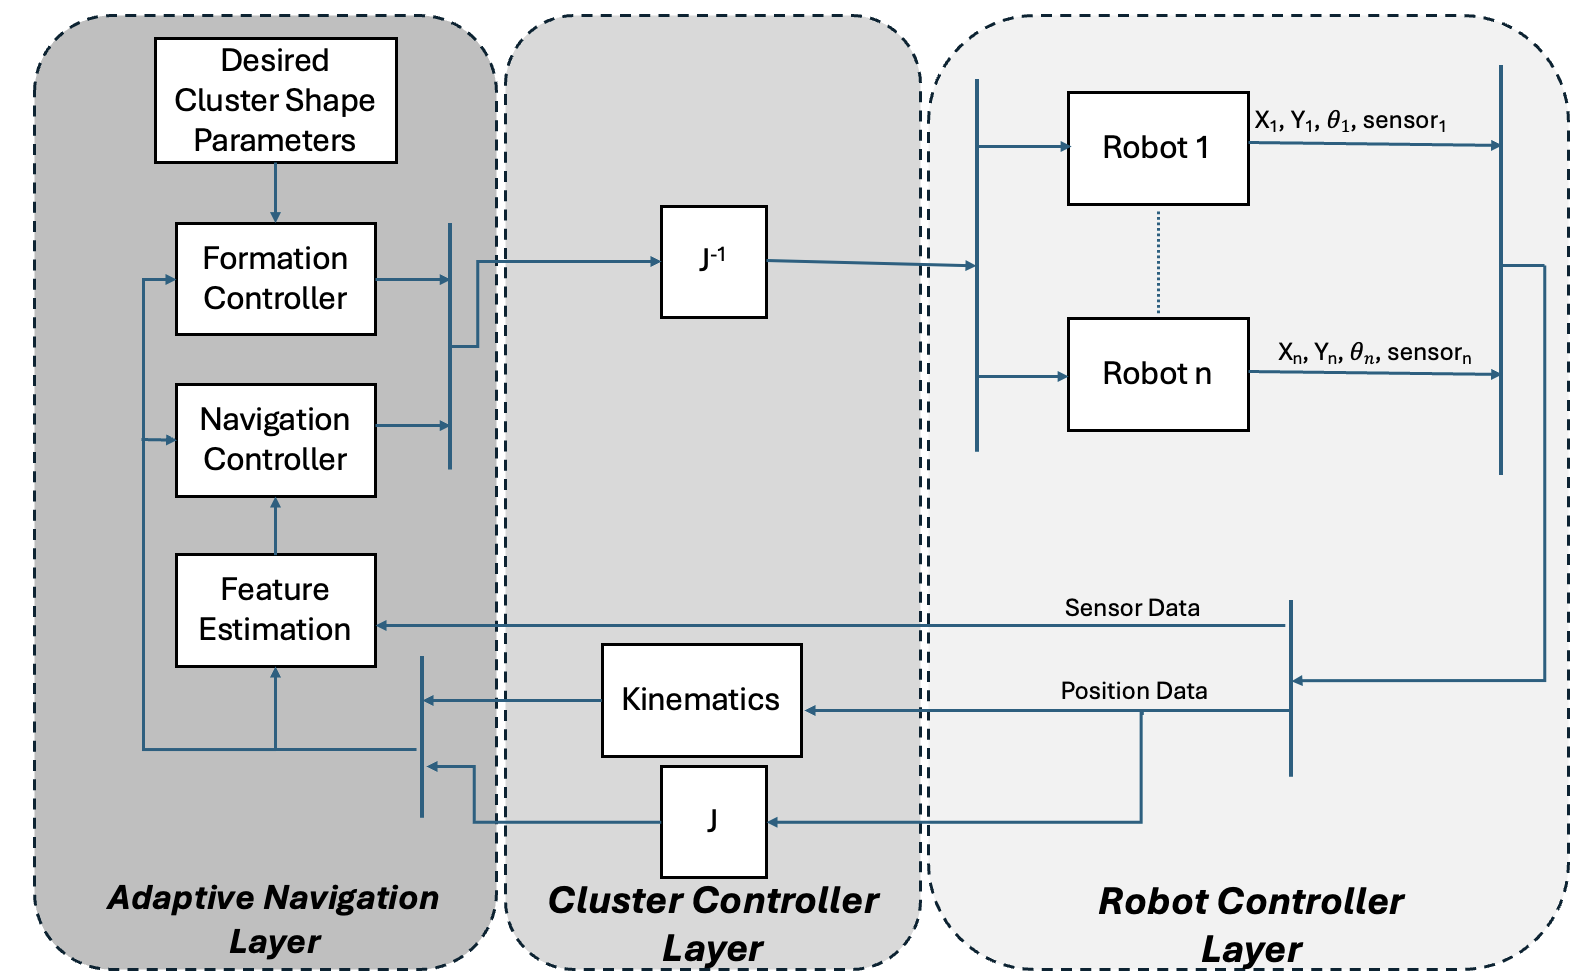
\includegraphics[width=\columnwidth]{figures/control_architecture.png}
    \caption{Three-layer control architecture: adaptive navigation (left),
    cluster controller (center), and robot controller (right). The contents
    of the feature estimation and navigation controller blocks are new in
    this paper.}
    \label{fig:control_architecture}
\end{figure}

\begin{figure}[!tb]
    \centering
    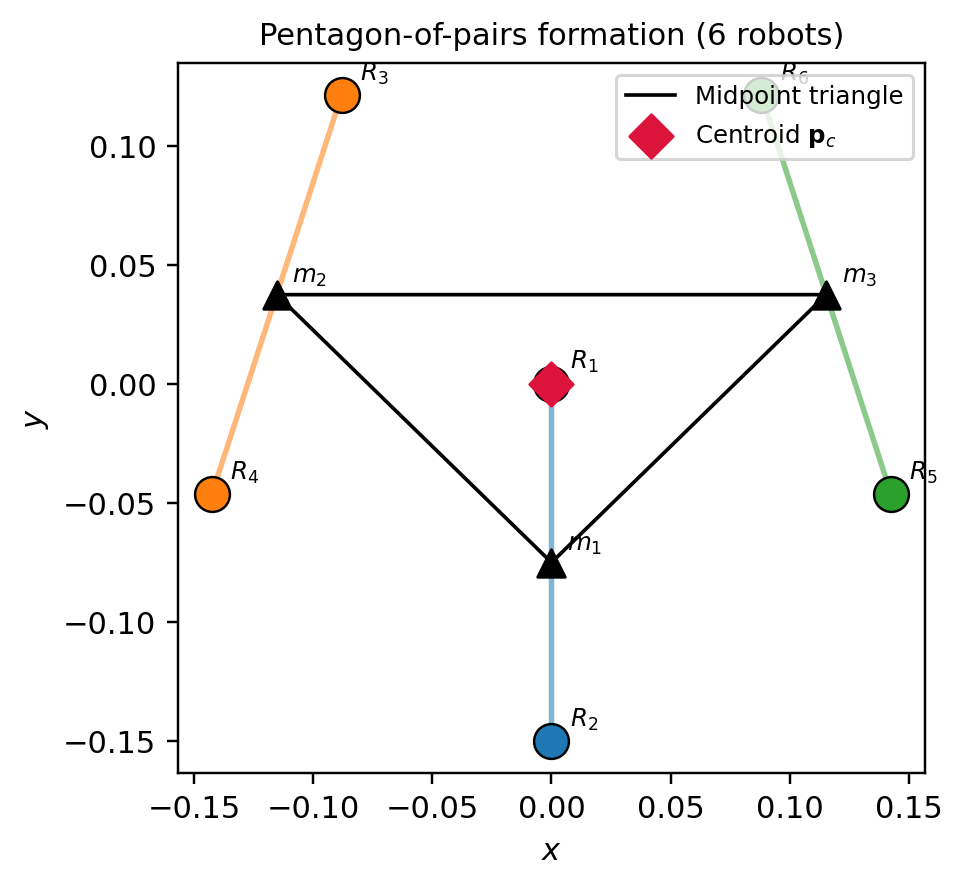
\includegraphics[width=0.8\columnwidth]{figures/pentagon_formation.png}
    \caption{Pentagon-plus-center formation. Robot 1 sits at the centroid
    $\mathbf{p}_c$ and robots 2 to 6 on a ring (dotted). The cluster
    variables shown are the pair separations $L_2$, $L_3$, $L_4$, a pair
    orientation $\theta_3$, the SAS parameters $(p, \beta, q)$ of the
    triangle of pair midpoints (squares), and the heading $\theta_c$.}
    \label{fig:pentagon}
\end{figure}

In the robot controller layer, each robot follows its velocity command
through the model that \cite{10} identified on the Decabot indoor
omnidirectional testbed \cite{31,32}. A robot reaches a share
$g = \rev{0.86}$ of its command after a delay $L = \rev{0.055}$~s, through
a first-order lag with time constant $\tau = \rev{0.02}$~s. It ignores
commands below a dead zone $v_c = 0.025$~m/s and is capped at 0.3~m/s. A
Python simulation integrates each robot's position by explicit Euler at the
control period $\Delta t = 0.1$~s. The simulation code and the scripts
behind every figure are available from the authors on request.

\subsection{The $D$ Tracker}
\label{sec:sep_controller}

The $D$ tracker is built for a mountain pass in $D$. Two minima are
joined by a trench that rises to a saddle point of $D$, the crest. On the
benchmark the trench is the separatrix and the minima are the flow saddles
(Fig.~\ref{fig:dg_fields}(b)). The tracker steers onto the trench, over
the crest, and down to the next minimum, with one channel across the trench,
one along it.

Across a trench $D$ curves upward, and along it $D$ can curve either way.
The tracker reads both directions from the eigenvectors of the fitted
Hessian, $\hat{\mathbf{H}}_{D,0}\mathbf{w}_j = \lambda_j \mathbf{w}_j$,
with $\|\mathbf{w}_j\| = 1$ and $\lambda_1 \leq \lambda_2$. The
eigenvector $\mathbf{w}_2$ points across the trench and $\mathbf{w}_1$
along it, signed by $\hat{\mathbf{v}}_0^\top \mathbf{w}_1 \geq 0$ to point
downstream, where $\hat{\mathbf{v}}_0 = (\hat{a}_1, \hat{b}_1)$ is the
measured flow at the centroid. This follows the height-ridge definition
of a trench \cite{33}, and on the benchmark the fitted eigenvectors lie
close to the true trench directions (Section~\ref{sec:dg_example}).

Away from the crest, both channels take Newton steps of the fitted
quadratic, $-\mathbf{w}_2^\top\hat{\mathbf{g}}_0/\lambda_2$ toward the
trench bottom and $|\mathbf{w}_1^\top\hat{\mathbf{g}}_0|/|\lambda_1|$
along it, which slows the cluster near the crest.

At the crest the along-trench gradient vanishes, and the measured flow
carries the cluster over instead. The tracker detects the crest as a
fitted saddle of $D$ whose stationary point lies inside the formation, a
crest set $\mathcal{B}$ where $\lambda_1\lambda_2 < 0$ and
\mbox{$\|\hat{\mathbf{H}}_{D,0}^{-1}\hat{\mathbf{g}}_0\| < c_{\mathrm{crest}}\,\rho$}.
The left side is the Newton step to the stationary point, so
$c_{\mathrm{crest}}$ is a fraction of the formation radius and needs no
knowledge of the field's scale.

Combining the two channels, the crest test selects the along-trench term,
\begin{equation}
    v_\parallel =
    \begin{cases}
        T\,\hat{\mathbf{v}}_0^\top \mathbf{w}_1,
            & \mathbf{p}_c \in \mathcal{B}, \\[6pt]
        \dfrac{|\mathbf{w}_1^\top \hat{\mathbf{g}}_0|}{|\lambda_1|},
            & \text{otherwise},
    \end{cases}
    \label{eq:vpar}
\end{equation}
and the centroid velocity command is
\begin{equation}
    \dot{\mathbf{p}}_c = k\Bigl[
    \underbrace{\mathrm{sat}(v_\parallel)\,\mathbf{w}_1}_{\text{along the trench}}
    + \underbrace{\mathrm{sat}\!\left(-\frac{\mathbf{w}_2^\top
      \hat{\mathbf{g}}_0}{\lambda_2}\right)\mathbf{w}_2}_{\text{across the trench}}\Bigr].
    \label{eq:d_law}
\end{equation}
Every term in the brackets is a distance, with $T$ one time unit in the
crest branch, so the navigation gain $k$ has units of inverse time. The
function $\mathrm{sat}(c) = c_{\max}\tanh(c/c_{\max})$ saturates each
channel at the distance $c_{\max}$, which caps the centroid speed at
$\sqrt{2}\,k\,c_{\max}$. It also bounds each Newton step where its
eigenvalue nears zero, and each eigenvalue in a denominator is floored at
$10^{-9}$ in magnitude, so no step divides by zero. Both branches of
$v_\parallel$ are nonnegative, so the along-trench motion never opposes
the flow, and where the fitted Hessian is definite the same law runs
unchanged.

The tracker stops at the end of the pass with the critical point test of
\cite{10}, which fires when the fitted flow has a saddle inside the
formation,
$\det\hat{\mathbf{J}}_0 < 0$ and
$\|\hat{\mathbf{J}}_0^{-1}\hat{\mathbf{v}}_0\| < \rho$, where $\hat{\mathbf{J}}_0$ is the fitted Jacobian at the centroid and
$\hat{\mathbf{J}}_0^{-1}\hat{\mathbf{v}}_0$ is the Newton step to the
stagnation point. The test uses only the zeroth- and first-order
coefficients, the least noisy the fit returns, and certifies a saddle of
the fitted linear flow, which on the benchmark is the flow saddle at the
end of the trench. Once it passes, the tracker
holds for the rest of the run with the attraction law of \cite{10},
$\dot{\mathbf{p}}_c = k\,\mathrm{sat}(-\hat{\mathbf{J}}_0^{-1}\hat{\mathbf{v}}_0)$
with $\mathrm{sat}$ applied to each component. Both read the measured
flow, so neither is objective.

\subsection{The $s_1$ Tracker}
\label{sec:s1_controller}

The fitted $\hat{s}_1$ is concave for any field and formation, so it
never shows the upward curvature a
trench has across it, and the $D$ tracker's Newton step has no counterpart
here. Both channels instead use $\nabla\hat{s}_1$ and the strain
eigenframe.

The trench tangent is a strain eigenvector (Section~\ref{sec:surrogates}),
and the tracker must choose between $\mathbf{e}_1$ and $\mathbf{e}_2$ at
every step. On the trench the transverse derivative of $s_1$ vanishes, so
$\nabla\hat{s}_1$ lies nearly along the trench away from a stationary
point. The tangent is the eigenvector most nearly parallel to it, signed
against a reference,
\begin{equation}
    \mathbf{t}_{\mathrm{raw}} =
    \arg\max_{\mathbf{e} \in \{\mathbf{e}_1, \mathbf{e}_2\}}
    \bigl\lvert \nabla\hat{s}_1^\top \mathbf{e} \bigr\rvert,
    \qquad
    \mathbf{t} = \mathrm{sgn}\bigl(\mathbf{t}_{\mathrm{ref}}^\top
    \mathbf{t}_{\mathrm{raw}}\bigr)\,\mathbf{t}_{\mathrm{raw}},
    \label{eq:tangent_select}
\end{equation}
where $\mathbf{t}_{\mathrm{ref}}$ is the previous step's tangent
(Fig.~\ref{fig:s1_channels}(a)). The first ride step has no previous
tangent, so the measured flow $\hat{\mathbf{v}}_0$ serves as
$\mathbf{t}_{\mathrm{ref}}$, the one non-objective input. After that,
objectivity holds at three levels. The quantities the tracker reads,
$\nabla\hat{s}_1$ and the strain eigenframe, are objective. The command
is rotationally equivariant only where the sign test is decisive: an
observer rotating at rate $\Omega$ turns the stored tangent by
$\Omega\,\Delta t$ between steps, which flips the sign only where
\mbox{$|\mathbf{t}_{\mathrm{ref}}^\top\mathbf{t}_{\mathrm{raw}}| <
\sin\Omega\,\Delta t$}, as at an eigenframe swap. The path, which a
rotating observer also sees carried by the frame's transport velocity,
matches across frames only empirically.

From the first step, the command pairs a constant-speed ride along
$\mathbf{t}$ with gradient descent across the trench,
\begin{equation}
    \dot{\mathbf{p}}_c = k\Bigl[
    \underbrace{\mathrm{sat}(c_{\max})\,\mathbf{t}}_{\text{along the trench}}
    + \underbrace{\mathrm{sat}\bigl(-g_\perp\,\mathbf{t}_\perp^\top
      \nabla\hat{s}_1\bigr)\,\mathbf{t}_\perp}_{\text{across the trench}}\Bigr],
    \label{eq:s1_law}
\end{equation}
with transverse gain $g_\perp$ and $\mathbf{t}_\perp$ the unit normal to
$\mathbf{t}$. As in (\ref{eq:d_law}) each bracketed term is a distance, so
$g_\perp$ carries units of length squared times time. The cluster rides at
speed $k\,c_{\max}\tanh 1$ throughout, and descends only across the
trench (Fig.~\ref{fig:s1_channels}(b)).

The ride speed does not depend on the slope, so the cluster crosses the
crest without the crest test the $D$ tracker needs. In incompressible flow
$s_1 = -r \leq 0$ reaches zero only at an isotropic point, where the
strain vanishes. In general such a point is isolated, so a crest is a
smooth saddle where $\nabla\hat{s}_1$ vanishes and the tangent rule is
least reliable. On the benchmark the shear strain vanishes identically, the
isotropic points form curves, and the crest sits on one at a kink of
$s_1$. There the tangent swaps eigenvector, and the rule follows the swap
with no dedicated test, since $\nabla\hat{s}_1$ stays large on either
side. Above the origin $u_x < 0$ and the trench follows $\mathbf{e}_2$,
an attracting OECS; below, $u_x > 0$ gives $\mathbf{e}_1$, a repelling
OECS.

The tracker stops at a minimum by a gradient test. The concave fit cannot
certify a minimum, but the fitted gradient tracks the true gradient even
where the fitted curvature has the wrong sign. Each end of the trench is
a true two-dimensional minimum of $s_1$, so a gradient that is small
against the depth suffices. Capture requires $\hat{s}_1 < 0$ and
$q = \rho\,\|\nabla\hat{s}_1\|/|\hat{s}_1| < q_{\mathrm{cap}}$, where $q$ is the fraction by which $\hat{s}_1$ changes across the
footprint. The ratio is dimensionless, so $q_{\mathrm{cap}}$ needs no
knowledge of the field's strain rate. It is large along the ride and wherever $\hat{s}_1$ nears zero, as at an isotropic point or a
gyre center, but small at any stationary point with $\hat{s}_1 < 0$, so
the test can also pass at a smooth crest. On the benchmark the crest sits
on an isotropic point, so only the minima pass. Once the test passes, the
tracker
drops the ride term and descends $\hat{s}_1$ for the rest of the run with
$\dot{\mathbf{p}}_c = -k\,\mathrm{sat}_{\mathrm{v}}(g_\perp\nabla\hat{s}_1)$,
where $\mathrm{sat}_{\mathrm{v}}(\mathbf{a}) =
\mathrm{sat}(\|\mathbf{a}\|)\,\mathbf{a}/\|\mathbf{a}\|$, with
$\mathrm{sat}_{\mathrm{v}}(\mathbf{0}) = \mathbf{0}$, saturates the
vector's magnitude and preserves its direction, which keeps the descent
independent of the coordinate axes.

\begin{figure}[!tb]
    \centering
    \includegraphics[width=\columnwidth]{figures/s1_channels_d14.png}
    \caption{The two channels of the $s_1$ tracker on the benchmark trench
    $x = 0$. (a) Tangent selection: the strain eigenframe, selected
    eigenvector heavy, with $\nabla\hat{s}_1$ in orange. The tangent is
    $\mathbf{e}_2$ on the attracting segment and $\mathbf{e}_1$ on the
    repelling one, swapping at the origin. (b) The command: an open-loop
    ride along $\mathbf{t}$ and a descent across it.}
    \label{fig:s1_channels}
\end{figure}

\subsection{Closed-Loop Behavior}
\label{sec:closed_loop}

Both trackers pull the cluster onto the trench through one saturated loop
across it, of the form \cite{10} analyzed on the same robots. With the
delay and gain of Section~\ref{sec:arch}, the sampled loop is
exponentially stable for loop gains below $1/(gL) = \rev{21.1}$ per unit
time, or \rev{16.1} with the lag included, and as a stable linear loop it
keeps the across-trench error bounded under a bounded estimate error
\cite{10}. The result is local and linearized, not a guarantee for the
full switched, saturated controller.

Neither channel is exactly linear. The $D$ tracker divides by the fitted
curvature, so its gain is $k$ times the ratio of true to fitted curvature
across the trench, $1/\sin^2\pi y_f$ on the benchmark. The gain is
$k = 3$ at the crest and exceeds the bound only within \rev{0.14} of the
saddles (Section~\ref{sec:dg_example}). The $s_1$ tracker's gain is
$k\,g_\perp\,\partial^2 s_1/\partial n^2$, or $3\pi^4 A\,|\cos\pi y_f|$
on the benchmark, which exceeds the bound for $|y| > \rev{0.19}$ and
reaches \rev{29} at the saddles. Each channel saturates a few thousandths
from the trench, which keeps any resulting oscillation in a narrow band.
At the end of the ride, the $D$ tracker's hold is the
attraction law of \cite{10}, so the cluster settles inside the friction
ring $v_c/k = \rev{0.008}$ around the fitted stagnation point.
Table~\ref{tab:params} collects the operating points.

\begin{table}[!t]
\caption{Operating points. The double-gyre column is non-dimensional,
with one time unit equal to one second of the Decabot's identified
dynamics. The ocean column uses the scaling of the Santa Barbara Channel
trial.}
\label{tab:params}
\centering
\begin{tabular}{llll}
\hline
Parameter & Double gyre & Ocean & Units \\
\hline
$k$                     & 3.0   & 1.94   & 1/time \\
$c_{\max}$              & 0.04  & 0.033  & length \\
$\rho$                  & 0.075 & 0.098  & length \\
$c_{\mathrm{crest}}$    & 0.1   & 0.1    & none \\
$g_\perp$               & 1.0   & 1.0    & length$^2\cdot$time \\
$q_{\mathrm{cap}}$      & 0.03  & 0.03   & none \\
robot $g$, $L$, $\tau$   & \rev{0.86}, \rev{0.055}, \rev{0.02} & 1, 0, 0 & --, time, time \\
dead zone $v_c$, cap     & 0.025, 0.3 & 0.002, 0.3 & length/time \\
\hline
\end{tabular}
\end{table}


\section{Double-Gyre Benchmark}
\label{sec:dg_bench}

\subsection{Setup}

The double-gyre experiments use the steady field of
Section~\ref{sec:dg_example} and the nominal formation, with ring radius
$\rho = 0.075$. Trials vary only the initial heading, set to zero in the
noise-free runs and drawn uniformly from $[0, 2\pi)$ in the Monte Carlo
sweeps, for up to 500 steps. The task is to ride the separatrix downstream
and capture the saddle at its end, $\mathbf{p}^*_1 = (0, -0.5)$; a run
that ends at $\mathbf{p}^*_2$ has ridden against the flow and fails. A
run acquires the separatrix at the first of ten consecutive
steps with its centroid within 0.05 of $x = 0$. Noise-free trials stop once
the centroid has stayed within 0.06 of a flow saddle for 20 consecutive
steps, while noisy trials succeed if the centroid comes within 0.06 of
$\mathbf{p}^*_1$. The formation straddles the separatrix when robots lie
on both sides of $x = 0$. Because losing the straddle is the failure
\cite{26} reports, we measure noise tolerance by retention, the fraction
of trials that succeed and never lose the straddle once they have it.

\subsection{Clean Runs}
\label{sec:disc_clean}

\begin{figure}[!tb]
    \centering
    \includegraphics[width=\columnwidth]{figures/traverse_vs_logic_c_seven_d14.png}
    \caption{$s_1$ tracker versus $D$ tracker from seven matched starts
    ($\bullet$), noise-free, at S1 $(-0.10, 0.30)$, S2 $(0.15, 0.25)$, S3 $(0, 0.35)$,
    S4 $(0, 0)$, S5 $(0, -0.25)$, S6 $(0.15, -0.15)$, and S7 $(0.10, -0.20)$,
    each ending at the downstream saddle ($\times$, squares). Shading marks
    the 0.1 cells from which a start reaches that saddle in at least 90\%
    (darker) or 50\% (lighter) of random headings, over \prelim{8000}
    noise-free starts per tracker.}
    \label{fig:traverse_vs_logic_c}
\end{figure}

\begin{figure}[!tb]
    \centering
    \includegraphics[width=\columnwidth]{figures/separatrix_formation_seven_d14.png}
    \caption{The six robots from start S1 (star) under both trackers,
    zoomed to the separatrix $x = 0$ (dashed): robot paths (thin), the
    centroid (heavy), and the formation at four instants.}
    \label{fig:formation}
\end{figure}

Without noise, both trackers acquire the separatrix, traverse it in the
same direction, and capture the downstream saddle from all seven matched
starts (Fig.~\ref{fig:traverse_vs_logic_c}). Three starts lie on the
separatrix, at heights $0.35$, $0$, and $-0.25$, and four lie off it by
$1.3\rho$ or $2\rho$, none straddling it at the first step. Both acquire
the separatrix in 0 to 10 steps. Runs from above the origin ride the upper
segment, an attracting OECS, through the isotropic point at the origin and
onto the lower, repelling one, with the formation straddling the
separatrix throughout (Fig.~\ref{fig:formation}). The $s_1$ tracker
crosses the origin on ordinary tangent selection.

The seven starts sample a wider basin (Fig.~\ref{fig:traverse_vs_logic_c},
shading). Near mid-height both trackers reach $\mathbf{p}^*_1$ in at least
90\% of headings from any start within \prelim{0.40} of the separatrix, more
than five formation radii, and the basin narrows to \prelim{0.25} at
$|y| = 0.2$. Farther out, the nearest trench need not be the separatrix.

Both hold $\mathbf{p}^*_1 = (0, -0.5)$ in all seven runs. The $D$ tracker
settles \rev{0.005} to \rev{0.006} from it, inside the friction ring of
Section~\ref{sec:closed_loop}, and the $s_1$ tracker within \rev{0.009}.
Where its gain exceeds the bound, the $s_1$ path wiggles about the
separatrix (Fig.~\ref{fig:formation}), a median \rev{0.004} from it below
$y = -0.19$ from S6 and S7, against under \rev{0.001} for the $D$
tracker.

\subsection{Behavior Under Noise}
\label{sec:disc_noise}

\begin{figure}[!tb]
    \centering
    \includegraphics[width=\columnwidth]{figures/noise_seven_starts_col_d14.png}
    \caption{Downstream-saddle success of both trackers from the seven starts of
    Fig.~\ref{fig:traverse_vs_logic_c}, one per row, \prelim{1000} trials per point,
    with each tracker's retention dashed. Ticks and labels mark the noise
    level at which retention falls to 50\%, and each inset marks the start
    (dot), the separatrix, and $\mathbf{p}^*_1$ (star). (a) Against
    $\sigma_{uv}$, $\sigma_p = 0$. (b) Against $\sigma_p$, $\sigma_{uv} = 0$.}
    \label{fig:flip_resolution}
\end{figure}

Both primitives sweep measurement and position noise separately from the
seven starts, at \prelim{1000} trials per noise level
(Fig.~\ref{fig:flip_resolution}), and both degrade smoothly as noise
grows.

The closed form of Section~\ref{sec:sensitivity} predicts where both must
fail. Each tracker steers on the second-order coefficients, and each pure
second derivative carries a standard deviation of
$2.53\,\sigma_{uv}/\rho^2$, which at $\rho = 0.075$ matches the largest
second derivative in the field, $\pi^3 A \approx 3.1$, near
$\sigma_{uv} = 0.007$. By $\sigma_{uv} = 0.01$ neither tracker keeps the
straddle in more than \prelim{60}\% of trials from any start. The same form
predicts how formation size moves the limit. From S3 and S4, the $D$
tracker's 50\% retention level rises by a factor of \prelim{5.0} and
\prelim{4.7} from $\rho = 0.05$ to $0.075$ and is never reached at
$\rho = 0.1125$, and the $s_1$ tracker's rises by \prelim{2.6} from
$\rho = 0.075$ to $0.1125$. Both beat the factor of 2.25 the coefficient
noise alone predicts, since a wider ring also straddles a larger offset,
so over this range the truncation error has not yet set the limit.

The $D$ tracker tolerates more noise from every start, under both noise
types. Against measurement noise its 50\%
retention level is \prelim{4.4} to \prelim{5.6} times the $s_1$ tracker's above
the origin, \prelim{3.5} times at it, and \prelim{1.3} to \prelim{1.5} times from S6
and S7, and from S5 its retention never falls to 50\%. Against position
noise the ratios are \prelim{2.8} to \prelim{4.9} and \prelim{1.3} to \prelim{1.4}.
Only from S6 and S7 do the retention curves cross, near
$\sigma_{uv} = \prelim{0.005}$. Halving $g_\perp$, which brings the $s_1$
tracker's gain under the bound of Section~\ref{sec:closed_loop}
everywhere, changes its retention by at most \prelim{2.3} points.

The $s_1$ tracker's main failure is a reversal: at
$\sigma_{uv} = 0.002$, \prelim{96} to \prelim{100}\% of its trials that miss
$\mathbf{p}^*_1$ end at $\mathbf{p}^*_2$. The $D$ tracker re-signs its
direction every cycle against the measured flow, while the $s_1$ tracker,
to stay objective, carries its sign forward. Near the saddles the
along-trench slope $\pi^3 A|\sin\pi y_f|$ that tangent selection relies on
goes to zero, so one noisy step can select the transverse eigenvector and
leave the next sign arbitrary. The chance of a first reversal per riding
step is \prelim{0.13} in the top tenth of the separatrix and
\prelim{0.002} to \prelim{0.004} midway.

The $D$ tracker's smaller margin from S6 and S7 comes from its fitted
Hessian, whose across-trench curvature falls short near the saddles
(Section~\ref{sec:dg_example}), so noise can make it definite before the
cluster reaches the separatrix. At $\sigma_{uv} = 0.005$ this happens in \prelim{95}\% and
\prelim{86}\% of trials from S6 and S7, which meet the separatrix near
$y = -0.30$, and only \prelim{32}\% and \prelim{38}\% of those trials reach
$\mathbf{p}^*_1$, against \prelim{85}\% and \prelim{81}\% of the rest. From S1
and S2, which meet it inside $|y| < 0.25$, the same happens in \prelim{75}\%
and \prelim{84}\% of trials without changing success.

\subsection{Behavior Under a Rotating Observer}
\label{sec:rotating}

\begin{figure}[!tb]
    \centering
    \includegraphics[width=\columnwidth]{figures/objectivity_rotating_d14.png}
    \caption{Rotating-observer trial from S1 (star), $10^4$ trials per
    frame, pulled back to inertial coordinates. Lines are mean paths with
    one standard deviation shaded, and squares are median final
    positions. Pentagons show heading-zero runs at $\Omega = \pm 0.18$.
    Only the $D$ tracker's path depends on the frame.}
    \label{fig:oecs_objectivity}
\end{figure}

A cluster can sense the water without error and still see the flow from a
rotating frame, when each robot adds its own velocity, differenced from
position fixes in drifting axes, to the water velocity it senses. The flow the cluster measures is then
$\mathbf{v}'(\mathbf{p}', t) = \mathbf{Q}\mathbf{v}(\mathbf{Q}^\top \mathbf{p}')
+ \Omega\,(-y', x')^\top$, the physical flow seen in rotated axes plus the transport velocity of a
frame rotating at rate $\Omega$, clockwise for $\Omega > 0$.

Both trackers start from S1 on the noise-free double gyre in the inertial
frame and in frames rotating at $\Omega = \pm 0.10$ and $\pm \rev{0.18}$,
with $10^4$ trials of random heading per frame, each stopping once its
centroid stalls or after 500 steps. The frame carries
$\mathbf{p}^*_1$ at $0.5|\Omega|$, and the $s_1$ capture delivers at most
$g\,k\,c_{\max} = \rev{0.103}$, so it can hold $\mathbf{p}^*_1$ only while
$|\Omega| < \rev{0.21}$. The faster rate stays \rev{13}\% inside that
bound.

The $s_1$ tracker follows the same path in every frame
(Fig.~\ref{fig:oecs_objectivity}, right), with a median largest offset
from the separatrix of \rev{0.010} in the inertial frame and at most
\rev{0.015} in the rotating ones. No trial loses the straddle, and every
trial holds $\mathbf{p}^*_1$, ending \rev{0.012} to \rev{0.015} from it.
Its channels and capture test use quantities a rotation leaves invariant,
its tangent seed agrees in every frame from S1, and its across-trench
feedback absorbs the frame's transport velocity, so the match is empirical
rather than exact.

The $D$ tracker's path depends on the frame
(Fig.~\ref{fig:oecs_objectivity}, left). Its median largest offset is
\rev{0.004} in the inertial frame, \rev{0.035} at $|\Omega| = 0.10$, and
\rev{0.063} at $|\Omega| = 0.18$, where \rev{28} to \rev{32}\% of trials
lose the straddle, the failure \cite{26} reports. The frame's added
vorticity $2\Omega$ shifts $D'$ by (\ref{eq:D_not_objective}). On the
separatrix the added term $\Omega\omega$ vanishes, but its transverse
gradient $2\pi^3 A\sin\pi y_f$ does not, and against the trench's
curvature $2\pi^6 A^2$ it moves the trench by
$\Omega\sin(\pi y_f)/(\pi^3 A)$, \rev{0.032} and \rev{0.058} at the origin,
close to the measured offsets. The transport velocity also moves the
fitted stagnation point $0.5|\Omega|/(\pi^2 A)$ from $\mathbf{p}^*_1$,
which the hold trails by $0.5|\Omega|/(g\,k)$. At $|\Omega| = 0.10$ the $D$ tracker ends a median
\rev{0.072} from $\mathbf{p}^*_1$, against \rev{0.012} for the $s_1$
tracker, and at $0.18$, where the shift reaches \rev{0.091}, beyond $\rho$,
it ends \rev{0.138} away.

\subsection{Beyond the Steady Gyre}
\label{sec:beyond}

\begin{figure*}[!tb]
    \centering
    \includegraphics[width=\textwidth]{figures/beyond_steady_d14.png}
    \caption{Each tracker rides a trench of its own field. Separatrices
    (black), the true trenches of $D$ and $s_1$ (thin), and one noise-free
    ride of each tracker (heavy) from S1 on the gyres and from B2, on the
    separatrix, on the jet; filled end markers reached the downstream
    saddle. (a) On the steady gyre the curves coincide. (b, c) Bending the
    separatrix bows both trenches past it. (d) On the Bickley jet the $s_1$
    trench runs nearly flat below the separatrix.}
    \label{fig:beyond}
\end{figure*}

\begin{table}[!t]
\caption{Noise-free outcomes beyond the steady gyre, $D$/$s_1$, in
percent of all trials from the seven starts: success, retention against
the separatrix (Ret.) and against the tracker's own true trench (Own),
reversal, and the median fitted $|\hat{\omega}|/2\hat{r}$ along the
ride.}
\label{tab:beyond}
\centering
\footnotesize
\setlength{\tabcolsep}{2.5pt}
\begin{tabular}{lccccc}
\hline
Field & Succ. & Ret. & Own & Rev. & $|\hat{\omega}|/2\hat{r}$ \\
\hline
Steady gyre                        & 100/100 & 100/100 & 100/100 & 0/0 & \prelim{0.01}/\prelim{0.02} \\
Time-periodic, $\epsilon = 0.1$    & \prelim{97}/\prelim{96} & \prelim{97}/\prelim{61} & & \prelim{3}/\prelim{4} & \prelim{0.11}/\prelim{0.07} \\
Time-periodic, $\epsilon = 0.25$   & \prelim{41}/\prelim{62} & \prelim{13}/\prelim{15} & & \prelim{15}/\prelim{26} & \prelim{0.10}/\prelim{0.20} \\
Bent, $\delta = 0.1$               & \prelim{71}/\prelim{100} & \prelim{67}/\prelim{29} & \prelim{71}/\prelim{70} & 0/$<$1 & \prelim{0.25}/\prelim{0.33} \\
Bent, $\delta = 0.2$               & \prelim{51}/\prelim{62} & \prelim{8}/\prelim{9} & \prelim{50}/\prelim{26} & 0/\prelim{9} & \prelim{0.52}/\prelim{0.53} \\
Bickley jet                        & \prelim{9}/0 & 0/0 & & \prelim{20}/0 & \prelim{0.61}/\prelim{0.60} \\
\hline
\end{tabular}
\end{table}

The steady double gyre is kind to both trackers. Its shear strain
vanishes, its separatrix is straight and still, and the rotation on the
separatrix vanishes, so both trenches lie exactly on it
(Fig.~\ref{fig:beyond}(a)). Three further fields take these properties
away a few at a time. Each runs without noise from the seven starts, with
\prelim{500} trials of random heading per start (\prelim{300} on the bent
gyre). The time-periodic member of
the family of \cite{14}, with period 10, swings the separatrix sideways at
up to 0.063 for $\epsilon = 0.1$ and 0.157 for $\epsilon = 0.25$ and puts
shear and rotation on it. A bent gyre, constructed here, replaces $x_f$ by
$x_f + \delta\sin\pi y_f$ in the stream function $A\sin\pi x_f\sin\pi y_f$
of (\ref{eq:dg_u}), which stays steady and incompressible but bows the
separatrix by $\delta$. A Bickley jet \cite{34}
with stream function
$-UL\tanh(y/L) + cy + UL\epsilon\,\mathrm{sech}^2(y/L)\cos k(x + 0.5)$,
$U = 0.3$, $L = 0.2$, $c = 0.3U$, $\epsilon = 0.3$, and $k = 2\pi$, seen in
the frame of its wave, has cat's-eye eddies bounded by U-shaped
separatrices, along most of which rotation exceeds strain.

Each tracker rides a trench of its own field, which marks the separatrix
only where strain outweighs rotation on it (Fig.~\ref{fig:beyond}). On the bent gyre the trench of $D$ bows up to
0.041 and 0.078 past the separatrix and the trench of $s_1$ up to 0.085
and 0.155. Scored against its own trench, the $s_1$ tracker keeps the
straddle in \prelim{70}\% of trials at $\delta = 0.1$ instead of
\prelim{29}\% (Table~\ref{tab:beyond}), so it has not lost its curve but
rides a different one. Retention against the
separatrix falls as the median fitted $|\hat{\omega}|/2\hat{r}$ along the
ride rises, from \prelim{97}\% near 0.1 to \prelim{29} to \prelim{67}\% near 0.3
and at most \prelim{9}\% above 0.5. On the Bickley jet the $s_1$ rides end a
median \prelim{0.007} from their own nearly flat trench, and the $D$
tracker, with no trench near much of it, succeeds in \prelim{9}\% of
trials.

Two failures have other causes. On the time-periodic gyre at
$\epsilon = 0.1$ the $s_1$ tracker keeps the straddle in only \prelim{61}\%
of trials, and every successful trial that loses it does so within 0.1 of
the crest, where the strain on the separatrix falls to
$\pi A\epsilon = 0.031$. There $s_1$ is nearly flat across the
moving trench, and its slope-driven channel cannot keep up, while the $D$
tracker's Newton step, a distance, does not weaken. At $\epsilon = 0.25$
the separatrix outruns the $g\,k\,c_{\max} = \rev{0.103}$ either channel
can deliver. On the bent gyre the $D$ tracker also fails from S6 and S7,
which the bend leaves \rev{3.2}$\rho$ and \rev{2.4}$\rho$ from the
separatrix, by acquiring the nearer bottom-wall trench instead.

Because $|\hat{\omega}|/2\hat{r}$ uses only first-order coefficients, a
cluster can compute it as it rides and flag an unreliable trench, provided
its heading is referenced to an inertial frame.

\section{Santa Barbara Channel Trial}
\label{sec:ocean}

\subsection{Setup}
\label{sec:ocean_sim}

The ocean experiment uses the public HFRNet U.S.~West Coast surface-current
product for the Santa Barbara Channel on its 2~km grid \cite{35,36}, with
the record of \cite{26}: 29 hourly frames from May 16, 2012 08:00 GMT to
May 17, 2012 12:00 GMT, in the same channel and month used by \cite{29}.
Radar coverage is partial, with 74 to 87\% of the water cells valid in
each frame. Missing cells, including land inside the coverage, are filled
by linear interpolation, the field is zero beyond valid data, and
interpolation is bilinear in space, linear in time.

The simulation maps $[-0.65, 0.65]^2$ onto a square centered on
$(34.2^{\circ}\mathrm{N}, 120.4^{\circ}\mathrm{W})$, with one length unit
of 51.4~km and one time unit of 6000~s, a uniform dilation once longitude
is scaled by $\cos(34.2^{\circ})$. Each control step advances
the field by 600~s, so the 168-step trial covers the record and any vessel
delay or lag is negligible (Table~\ref{tab:params}). The speed cap
$\sqrt{2}\,k\,c_{\max}$ is then 0.78~m/s, within reach of a small
autonomous surface vessel. Both trackers start north of the channel
entrance at $(34.38^{\circ}\mathrm{N}, 120.41^{\circ}\mathrm{W})$ with
heading $335^\circ$. A run ends at the end of the record or at landfall,
when any robot lies over land on the Natural Earth 1:10 million coastline,
so filled land cells reach only fits near the coast.

An offline FTLE field, available to neither controller, serves as the
Lagrangian reference \cite{14}. It advects a seed grid four times finer
than the data by fourth-order Runge-Kutta at 600~s steps, with land held
at zero velocity. The water points at or above the 95th percentile of the
24-h forward field anchored at the record start form a high-FTLE band that
contains the dominant ridge (Fig.~\ref{fig:ocean_ftle}), and a distance to
the ridge here means a distance to this band. Recomputing a 12-h field at
four anchor times shows that this ridge persists while the finer structure
downstream evolves. The pentagon is enlarged to $\rho = 0.098$, 5.0~km,
so that it spans the several grid cells a quadratic fit needs. The radius $\rho$ and gain $k$ are tuned
against the FTLE reference, as they set when the cluster reaches the
evolving ridge's bifurcation and so which branch it meets.

\subsection{Results}
\label{sec:disc_ocean}

\begin{figure*}[!tb]
    \centering
    \includegraphics[width=\textwidth]{figures/ocean_progression_2km.png}
    \caption{$D$ and $s_1$ tracker paths from a single shared start at
    (a) 7, (b) 14, (c) 21, and (d) 28~h, each drawn up to that time, over
    the 24-h forward FTLE field anchored at the record start. Both follow
    the dominant ridge from the channel entrance to the bifurcation and take
    the same branch past it.}
    \label{fig:ocean_ftle}
\end{figure*}

Both trackers follow the dominant ridge of the forward FTLE field from the
channel entrance to the bifurcation and take the same branch past it
(Fig.~\ref{fig:ocean_ftle}). This agreement is not built
in, as the field is divergent and not vorticity-free. Along both paths
the fit is strain-dominated, with $\hat{D} < 0$ on about 80\% of
steps and a median $|\hat{\omega}|/2\hat{r}$ of 0.15 to 0.20 from 7 to 21~h.
$D$ is then close to $s_1 s_2 = \mu^2 - r^2$, where divergence enters only
as $\mu^2$, a tenth to a fifth of $r^2$. Divergence enters
$s_1 = \mu - r$ linearly, however, so the 1.3~km mean separation of the
two paths is an observation on this record.

The $s_1$ tracker also types what it rides. Its tangent followed
$\mathbf{e}_2$, an attracting OECS, on 34 of 42 steps from 7 to 14~h, and
$\mathbf{e}_1$ on 37 of 42 steps from 14 to 21~h. A 12-h backward FTLE
field anchored at 14~h marks attracting structures and checks both
segments. Over 7 to 14~h the $s_1$ path ran a mean \rev{1.7}~km from its
top 5\%, against \rev{5.6}~km for the $D$ path. Over 14 to 21~h it ran
\rev{6.5}~km from that band and \rev{2.0}~km from the forward one. In this
divergent field a trench along $\mathbf{e}_1$ is a repelling OECS only
where it is also a ridge of $s_2$, which held on 49\% of the later steps.

The two trackers differ in speed early on. From 2 to 6.5~h the $s_1$
tracker crossed a patch near the entrance where rotation and divergence
rival the strain ($\hat{D} > 0$ on 70\% of steps), switching tangents 12
times in 27 steps, and in the first 7~h it made 2.1~km of net progress
against 8.4~km for the $D$ tracker. Past the patch both kept pace, a mean
1.6 and 2.1~km from the ridge. The $D$ tracker reached land at 23~h. The
$s_1$ tracker drifted 3.8~km off the weakening ridge in the southern
channel, as the robots of \cite{26} also did, and remained at sea at 28~h.

Small changes to the shared start show which of these behaviors are
reliable. Over 100 runs that move the start by up to 1~km, turn the
heading by up to $15^\circ$, and scale $\rho$, $k$, and $c_{\max}$ by up
to 5\%, both trackers stay on the same ridge, a median \rev{1.5} and
\rev{0.9}~km from it, but ride it in different directions. The $D$
tracker signs its direction against the measured flow every cycle, so it
always rides downstream: \rev{99} of its runs reach the southern channel
and \rev{66} land at the island. The $s_1$ tracker signs each tangent
against the one before it, and in the patch near the entrance that chain
breaks. There the strain eigenframe swaps, and a swap compares the new
tangent with a perpendicular old one, so its sign is close to a coin toss.
In \rev{98} runs the $s_1$ tracker turned against the flow at a median
\rev{2.5}~h, where the fitted $|\hat{\omega}|/2\hat{r}$ had risen to
\rev{0.46} against \rev{0.27} along the $D$ rides, then rode the ridge
north to the mainland. The shared start of Fig.~\ref{fig:ocean_ftle} is
the one setting of the \rev{101} tested in which the tosses came out
downstream. This is the reversal of the double-gyre runs, set off by
rotation instead of noise, and the ratio $|\omega|/2r$ flags where it
happens.

\section{Limitations and Future Work}
\label{sec:disc_limits}

Cluster space control is centralized and needs global state and reliable
high-bandwidth communication \cite{30}. Unlike distributed or
event-triggered consensus protocols \cite{37}, the estimator gathers all six
readings on one processor, so the claims here are for small clusters with
ample bandwidth.

Both trackers follow trenches of their own fields, which leave a
separatrix once the rotation on it rivals the strain
(Section~\ref{sec:beyond}). The $s_1$ tracker can reverse wherever its
eigenframe swaps, and its capture test can pass at a smooth crest. The
$D$ tracker's fitted Hessian omits the third-derivative terms that
dominate near the saddles, and the tracker is not objective.

The evaluation is kinematic simulation without flow advection, and the
ocean trial uses one record without added noise. In general neither
instantaneous Eulerian field is guaranteed to mark a Lagrangian material
transport structure \cite{19}. No head-to-head against \cite{26,27,28} or
\cite{29} was run. Their robots ride the flow and steer relative to it,
while ours command velocity over ground, so a fair comparison needs one
advection model for both, and their analyses assume a straddling start
that four of our seven starts do not provide. The no-advection premise is
exact on the planned Decabot hardware, where the field is only encoded
\cite{32}, but untested in a physical flow.

Future work targets three extensions. First, a fit from more than six
robots becomes least squares, which averages the measurement noise and
leaves a residual that, where the truncation error is small, estimates
that noise online. A cluster could then detect the high-noise regime in
which neither tracker is reliable. Second, the
$s_1$ tracker could take as its tangent the strain eigenvector nearest the
previous tangent. That rule does not rest on the along-trench slope and
could carry the direction through the eigenframe swaps behind both kinds
of reversal. Finally, a cubic
fit from ten robots off any common cubic curve would recover the third
derivatives on which the true $\mathbf{H}_D$ and the transverse curvature
of an $s_1$ trench depend.

\section{Conclusion}

This paper has shown that six robots sampling at once can fit a local
quadratic model of a planar flow, which gives the velocity gradient as a
field over the formation. Two surrogate fields read from that fit, the
Jacobian determinant $D$ and the smaller strain eigenvalue $s_1$, have
trenches that, in the tested environments, lie closest to coherent
structures where strain dominates rotation, and on each we built an adaptive navigation primitive that acquires
and rides those trenches from instantaneous measurements, with no
integration horizon and no pre-straddling. Without noise, both traverse
the double-gyre separatrix from every start and hold the downstream
saddle. The $D$ tracker withstands more measurement and position noise
from every start tested, while the $s_1$ tracker, built from objective
quantities, alone holds its path under a rotating observer. On the Santa
Barbara Channel record both acquire the dominant transport corridor, but
under small changes to the start only the $D$ tracker keeps its
direction. Choosing between them is therefore a trade-off: rotational
robustness favors the $s_1$ tracker, while noise tolerance and directional
reliability favor the $D$ tracker. A cluster with an absolute heading
reference, such as a compass or GNSS, gives up little by carrying the $D$
tracker and can trust its own rotation-to-strain ratio.

\begin{thebibliography}{99}
\itemsep 0pt plus 0.2pt
\parskip 0pt
\bibitem{1} J. Cortés and M. Egerstedt, ``Coordinated control of multi-robot
systems: A survey,'' \textit{SICE J. Control Meas. Syst. Integr.},
vol. 10, no. 6, pp. 495--503, 2017.

\bibitem{2} T. Adamek, C. A. Kitts, and I. Mas, ``Gradient-based cluster space
navigation for autonomous surface vessels,'' \textit{IEEE/ASME Trans.
Mechatronics}, vol. 20, no. 2, pp. 506--518, 2015.

\bibitem{3} C. A. Kitts, R. T. McDonald, and M. A. Neumann, ``Adaptive
navigation control primitives for multirobot clusters: Extrema finding,
contour following, ridge/trench following, and saddle point station keeping,''
\textit{IEEE Access}, vol. 6, pp. 17625--17642, 2018.

\bibitem{4} P. Ögren, E. Fiorelli, and N. E. Leonard, ``Cooperative control
of mobile sensor networks: Adaptive gradient climbing in a distributed
environment,'' \textit{IEEE Trans. Autom. Control}, vol. 49, no. 8,
pp. 1292--1302, 2004.

\bibitem{5} L. Briñón-Arranz, A. Renzaglia, and L. Schenato, ``Multirobot
symmetric formations for gradient and Hessian estimation with application to
source seeking,'' \textit{IEEE Trans. Robot.}, vol. 35, no. 3,
pp. 782--789, 2019.

\bibitem{6} R. T. McDonald et al., ``Navigation of
scalar fronts with multirobot clusters in simulation and experiment,''
\textit{IEEE Syst. J.}, vol. 14, no. 3, pp. 3755--3766, 2020.

\bibitem{7} R. T. McDonald, C. A. Kitts, and M. A. Neumann, ``Experimental
implementation and verification of scalar field ridge, trench, and saddle
point maneuvers using multirobot adaptive navigation,'' \textit{IEEE Access},
vol. 7, pp. 62950--62961, 2019.

\bibitem{8} A. Okubo, ``Horizontal dispersion of floatable particles in the
vicinity of velocity singularities such as convergences,'' \textit{Deep-Sea
Res.}, vol. 17, no. 3, pp. 445--454, 1970.

\bibitem{9} P. Keramea, K. Spanoudaki, G. Zodiatis, G. Gikas, and
G. Sylaios, ``Oil spill modeling: A critical review on current trends,
downscaling, and applications,'' \textit{J. Mar. Sci. Eng.}, vol. 9,
no. 2, art. 181, 2021.

\bibitem{10} C. Waight and C. A. Kitts, ``Adaptive navigation of multirobot
systems to critical points in 2D vector fields in simulation and
experiment,'' submitted for publication.

\bibitem{11} T. Peacock and G. Haller, ``Lagrangian coherent structures: The
hidden skeleton of fluid flows,'' \textit{Phys. Today}, vol. 66, no. 2,
pp. 41--47, 2013.

\bibitem{12} M. Serra et al., ``Search and rescue at sea aided by hidden flow
structures,'' \textit{Nat. Commun.}, vol. 11, no. 1, p. 2525, 2020.

\bibitem{13} G. Haller and G. Yuan, ``Lagrangian coherent structures and mixing
in two-dimensional turbulence,'' \textit{Physica D}, vol. 147, no. 3-4,
pp. 352--370, 2000.

\bibitem{14} S. C. Shadden, F. Lekien, and J. E. Marsden, ``Definition and
properties of Lagrangian coherent structures from finite-time Lyapunov
exponents in two-dimensional aperiodic flows,'' \textit{Physica D}, vol. 212,
no. 3-4, pp. 271--304, 2005.

\bibitem{15} J. Weiss, ``The dynamics of enstrophy transfer in two-dimensional
hydrodynamics,'' \textit{Physica D}, vol. 48, no. 2-3, pp. 273--294, 1991.

\bibitem{16} J. C. R. Hunt, A. A. Wray, and P. Moin, ``Eddies, streams, and
convergence zones in turbulent flows,'' in \textit{Proc. Summer Program,
Center Turbul. Res.}, Rep. CTR-S88, pp. 193--208, 1988.

\bibitem{17} B.-L. Hua and P. Klein, ``An exact criterion for the stirring
properties of nearly two-dimensional turbulence,'' \textit{Physica D}, vol. 113,
no. 1, pp. 98--110, 1998.

\bibitem{18} C. Dong et al., ``Oceanic mesoscale eddies,''
\textit{Ocean-Land-Atmos. Res.}, vol. 4, p. 0081, 2025.

\bibitem{19} G. Haller, ``Lagrangian coherent structures,'' \textit{Annu. Rev.
Fluid Mech.}, vol. 47, pp. 137--162, 2015.

\bibitem{20} M. Serra and G. Haller, ``Objective Eulerian coherent
structures,'' \textit{Chaos}, vol. 26, no. 5, p. 053110, 2016.

\bibitem{21} P. J. Nolan, M. Serra, and S. D. Ross, ``Finite-time Lyapunov
exponents in the instantaneous limit and material transport,''
\textit{Nonlinear Dyn.}, vol. 100, no. 4, pp. 3825--3852, 2020.

\bibitem{22} T. D. Harms, S. L. Brunton, and B. J. McKeon, ``Lagrangian
gradient regression for the detection of coherent structures from sparse
trajectory data,'' \textit{R. Soc. Open Sci.}, vol. 11, no. 9,
p. 240586, 2024.

\bibitem{23} J. Das et al., ``Coordinated sampling of dynamic oceanographic
features with underwater vehicles and drifters,'' \textit{Int. J. Robot.
Res.}, vol. 31, no. 5, pp. 626--646, 2012.

\bibitem{24} S. McCammon et al., ``Ocean front detection and tracking using a
team of heterogeneous marine vehicles,'' \textit{J. Field Robot.}, vol. 38,
no. 6, pp. 854--881, 2021.

\bibitem{25} S. R. Ramp et al., ``Preparing to predict: the second autonomous
ocean sampling network (AOSN-II) experiment in the Monterey Bay,''
\textit{Deep-Sea Res. II}, vol. 56, no. 3-5, pp. 68--86, 2009.

\bibitem{26} M. Michini, M. A. Hsieh, E. Forgoston, and I. B. Schwartz,
``Robotic tracking of coherent structures in flows,'' \textit{IEEE Trans.
Robot.}, vol. 30, no. 3, pp. 593--603, 2014.

\bibitem{27} M. Michini, H. Rastgoftar, M. A. Hsieh, and S. Jayasuriya,
``Distributed formation control for collaborative tracking of manifolds in
flows,'' in \textit{Proc. Amer. Control Conf.}, pp. 3874--3880, 2014.

\bibitem{28} M. Michini, M. A. Hsieh, E. Forgoston, and I. B. Schwartz,
``Experimental validation of robotic manifold tracking in gyre-like flows,''
in \textit{Proc. IEEE/RSJ Int. Conf. Intell. Robots Syst.},
pp. 2306--2311, 2014.

\bibitem{29} D. Kularatne and M. A. Hsieh, ``Tracking attracting manifolds in
flows,'' \textit{Auton. Robots}, vol. 41, no. 8, pp. 1575--1588, 2017.

\bibitem{30} C. A. Kitts and I. Mas, ``Cluster space specification and control
of mobile multirobot systems,'' \textit{IEEE/ASME Trans. Mechatronics},
vol. 14, no. 2, pp. 207--218, 2009.

\bibitem{31} S. Tomer et al., ``A low-cost indoor testbed for multirobot
adaptive navigation research,'' in \textit{Proc. IEEE Aerosp. Conf.},
pp. 1--12, 2018.

\bibitem{32} C. Waight and C. A. Kitts, ``A functional indoor testbed for
multirobot adaptive navigation in vector field environments,'' in
\textit{Proc. ASME Int. Des. Eng. Tech. Conf.}, vol. 89251, 2025.

\bibitem{33} D. Eberly et al., ``Ridges for image analysis,''
\textit{J. Math. Imaging Vis.}, vol. 4, no. 4, pp. 353--373, 1994.

\bibitem{34} I. I. Rypina, M. G. Brown, F. J. Beron-Vera, H. Ko\c{c}ak,
M. J. Olascoaga, and I. A. Udovydchenkov, ``On the Lagrangian dynamics of
atmospheric zonal jets and the permeability of the stratospheric polar
vortex,'' \textit{J. Atmos. Sci.}, vol. 64, no. 10, pp. 3595--3610, 2007.

\bibitem{35} Coastal Observing Research and Development Center, Scripps
Inst. Oceanogr., ``Near-real time surface ocean velocity, U.S. West Coast,
2 km resolution,'' HFRNet, NOAA NCEI Accession
gov.noaa.nodc:IOOS-HFRadarRTVector, 2012. [Online]. Available:
\url{https://www.ncei.noaa.gov/thredds-ocean/fileServer/ioos/hfradar/rtv/2012/201205/USWC/}.
Accessed: Jul. 1, 2026.

\bibitem{36} E. Terrill et al., ``Data management and real-time distribution
in the HF-Radar National Network,'' in \textit{Proc. MTS/IEEE OCEANS},
Boston, MA, USA, Sep. 2006.

\bibitem{37} S. Zhang, J. Liu, W. Wang, and Z. Zhang, ``Bipartite
leader-following consensus of nonlinear switched multiagent systems under
model-depended dynamic event-triggered control,'' \textit{IEEE Syst. J.},
vol. 18, no. 2, pp. 1044--1055, 2024.

\end{thebibliography}

\end{document}

